%! TEX root = main.tex
This subsection presents our experiments with several new training strategies, including the annealing loss aggregation, cyclical learning rate, stochastic weight averaging, and the nonlinear conjugate-gradient method.

\subsubsection{Annealing Loss Aggregation}

We applied annealing loss aggregation described in section \ref{sec:loss-annealing} to the cases of $(N_l, N_n, N_{bs}) = (1, 16, 8192)$, $(2, 32, 8192)$, and $(3, 128, 8192)$.
The $\lambda$ parameter in the annealing algorithm is $0.1$ for all cases.
In all the comparisons, we refer to the original loss handling (i.e., equation \eqref{eq:total-residual}) as {\it even-weight aggregation} in the text and {\it naive sum} in the figures to save space.

\begin{figure}[hbt!]
    \centering%
    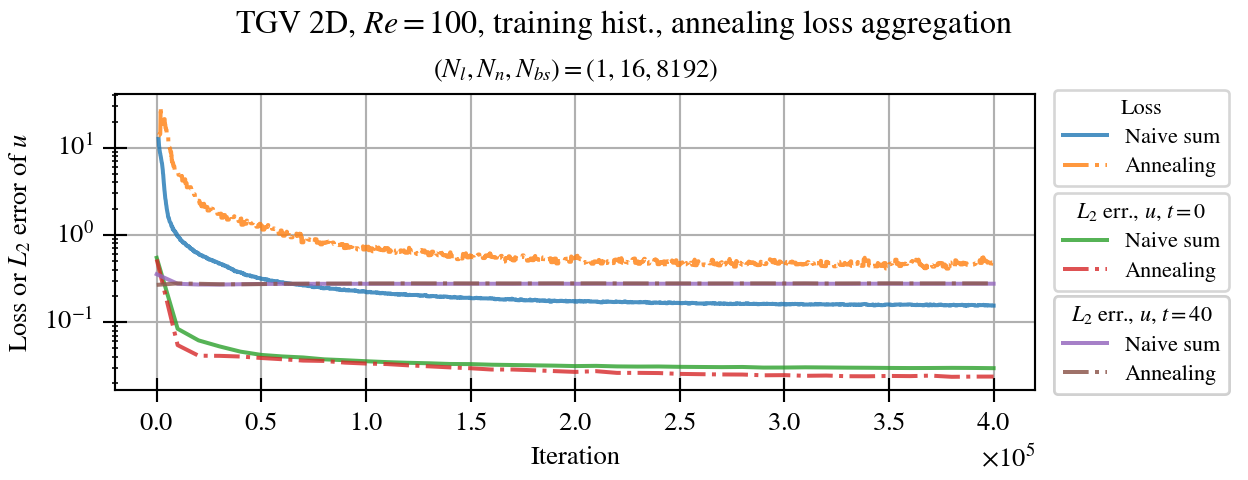
\includegraphics[width=0.9\linewidth]{tgv-2d-re100/annealing-tests/nl1-nn16-npts8192-steps}%
    \caption[%
        Annealing loss aggregation: loss and $L_2$ errors of $u$ v.s. iteration ($(N_l, N_n, N_{bs})=(1, 16, 8192)$)%
    ]{%
        Annealing loss aggregation: loss and $L_2$ errors of $u$ v.s. iteration ($(N_l, N_n, N_{bs})=(1, 16, 8192)$)%
    }\label{fig:annealing-tests-nl1-nn16-npts8192-steps}%
\end{figure}

\begin{figure}[hbt!]
    \centering%
    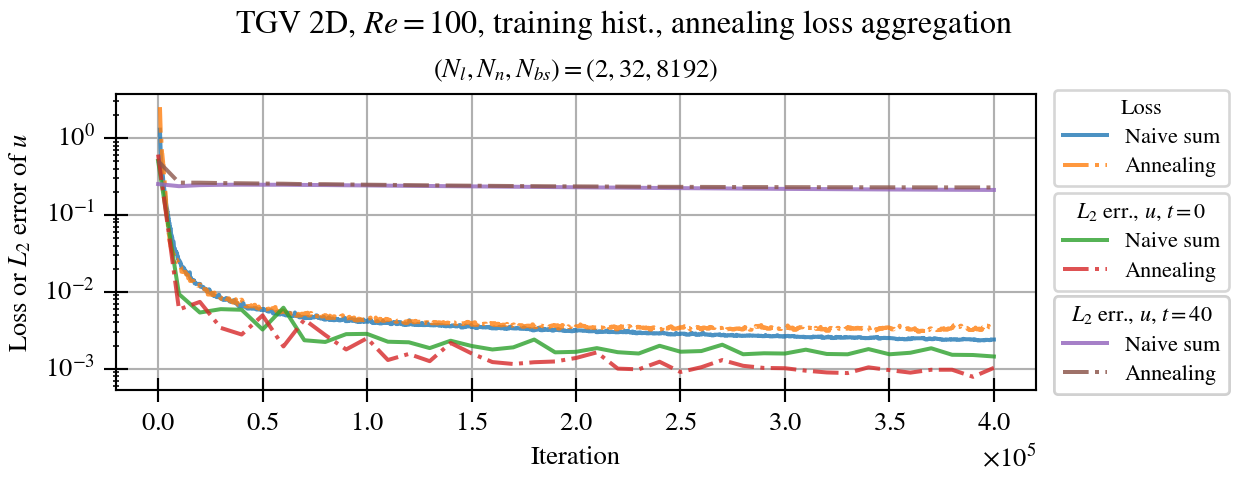
\includegraphics[width=0.9\linewidth]{tgv-2d-re100/annealing-tests/nl2-nn32-npts8192-steps}%
    \caption[%
        Annealing loss aggregation: loss and $L_2$ errors of $u$ v.s. iteration ($(N_l, N_n, N_{bs})=(2, 32, 8192)$)%
    ]{%
        Annealing loss aggregation: loss and $L_2$ errors of $u$ v.s. iteration ($(N_l, N_n, N_{bs})=(2, 32, 8192)$)%
    }\label{fig:annealing-tests-nl2-nn32-npts8192-steps}%
\end{figure}

\begin{figure}[hbt!]
    \centering%
    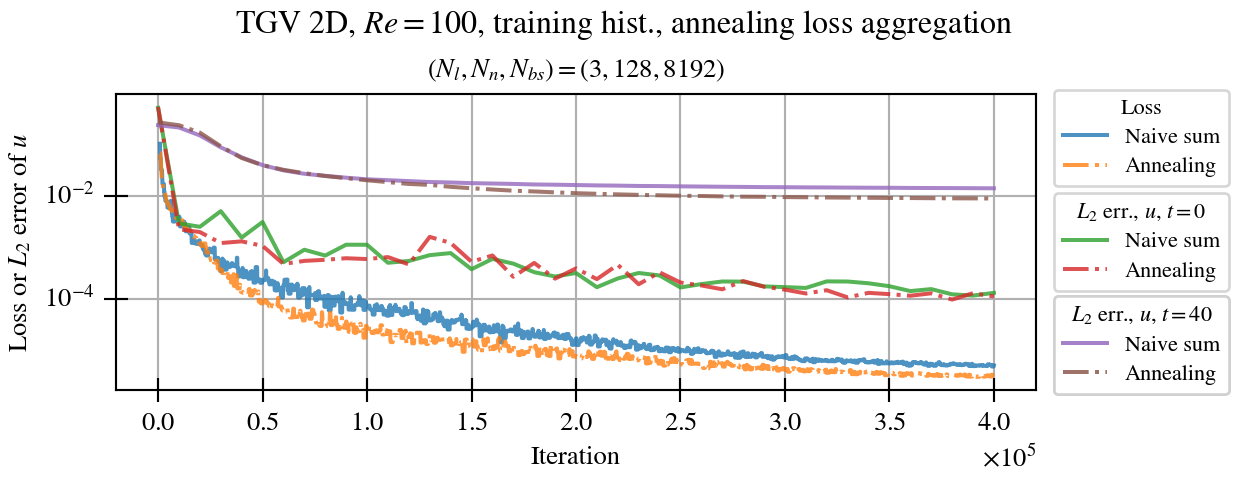
\includegraphics[width=0.9\linewidth]{tgv-2d-re100/annealing-tests/nl3-nn128-npts8192-steps}%
    \caption[%
        Annealing loss aggregation: loss and $L_2$ errors of $u$ v.s. iteration ($(N_l, N_n, N_{bs})=(3, 128, 8192)$)%
    ]{%
        Annealing loss aggregation: loss and $L_2$ errors of $u$ v.s. iteration ($(N_l, N_n, N_{bs})=(3, 128, 8192)$)%
    }\label{fig:annealing-tests-nl3-nn128-npts8192-steps}%
\end{figure}

Figures \ref{fig:annealing-tests-nl1-nn16-npts8192-steps}, \ref{fig:annealing-tests-nl2-nn32-npts8192-steps}, and \ref{fig:annealing-tests-nl3-nn128-npts8192-steps} show the convergence histories of the aggregated losses and errors of $u$.
An interesting observation is that, in figure \ref{fig:annealing-tests-nl1-nn16-npts8192-steps}, the evident gap in the losses of the two algorithms are not reflected in the errors of $u$.
The reason may be that the difference in the losses is due to the different weights of loss terms.
Annealing aggregation may assign a large weight to the IC loss and hence shows a higher aggregated loss.
Other than this observation, we did not observe quantitatively significant difference in both loss and errors between the two algorithms.

Figure \ref{fig:annealing-tests-final-sterrs} gives the comparison of the final $L_{2,sp-t}$ for both $u$ and $v$ velocity.
For simpler network architectures, $(1, 16, 8192)$ and $(2, 32, 8192)$, the final spatial-temporal errors are close.
The more complicated model, $(3, 128, 8192)$, shows visually obvious difference.
However, after examining the actual quantities, we consider them similar.
For example, in the $u$ velocity and with the case of $(3, 128, 8192)$, the even-weight aggregation has an error between $1e-2$ to $2e-2$, while the annealing algorithm has an error between $8e-3$ to $9e-3$.
The difference is just about $20\%$ smaller relative to the even-weight aggregation.
And this difference is even smaller in $v$ velocity.

\begin{figure}[hbt!]
    \centering%
    \includegraphics[width=0.9\linewidth]{tgv-2d-re100/annealing-tests/final-spatial-temporal-errors}%
    \caption[%
        Annealing loss aggregation: final spatial-temporal errors%
    ]{%
        Annealing loss aggregation: final spatial-temporal errors%
    }\label{fig:annealing-tests-final-sterrs}%
\end{figure}

We further examined the convergence with respect to the run times.
Annealing loss aggregation is more expensive as it involves evaluating the gradient of each single loss term with respect to model parameters.
As shown in figures \ref{fig:annealing-tests-nl1-nn16-npts8192-walltimes}, \ref{fig:annealing-tests-nl2-nn32-npts8192-walltimes}, and \ref{fig:annealing-tests-nl3-nn128-npts8192-walltimes}, the even-weight aggregation is considered to converge much faster in terms of the run time.
Though annealing aggregation shows a slightly better accuracy at the end of training for $(3, 128, 8192)$, the even-weight aggregation achieves slightly better losses and errors under a given, meaning a better accuracy-cost ratio.
Annealing loss aggregation's computational cost is about the double of the even-weight aggregation. 

\begin{figure}[hbt!]
    \centering%
    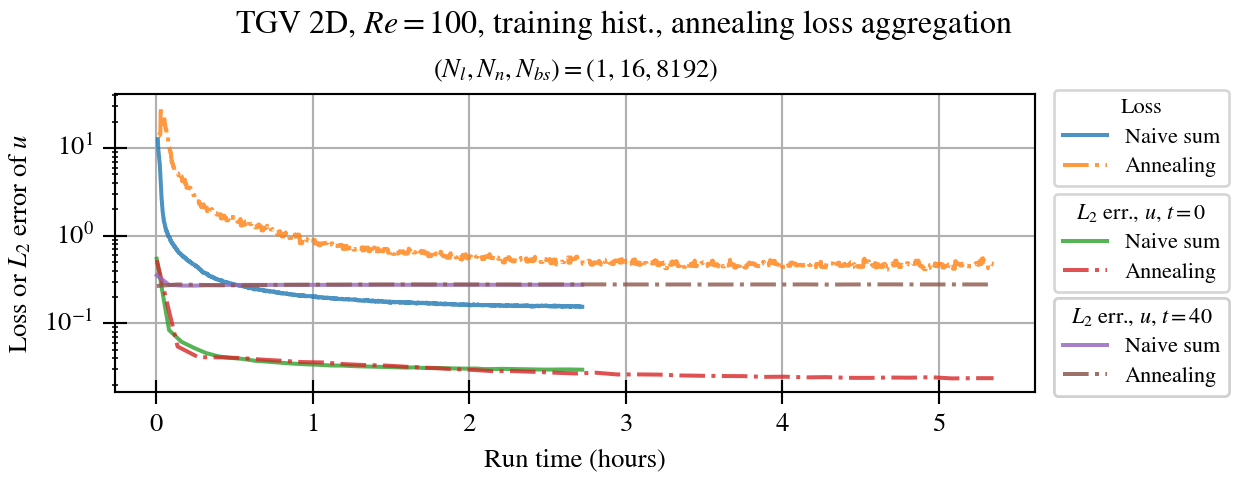
\includegraphics[width=0.9\linewidth]{tgv-2d-re100/annealing-tests/nl1-nn16-npts8192-walltimes}%
    \caption[%
        Annealing loss aggregation: loss and $L_2$ errors of $u$ v.s. wall time ($(N_l, N_n, N_{bs})=(1, 16, 8192)$)%
    ]{%
        Annealing loss aggregation: loss and $L_2$ errors of $u$ v.s. wall time ($(N_l, N_n, N_{bs})=(1, 16, 8192)$)%
    }\label{fig:annealing-tests-nl1-nn16-npts8192-walltimes}%
\end{figure}

\begin{figure}[hbt!]
    \centering%
    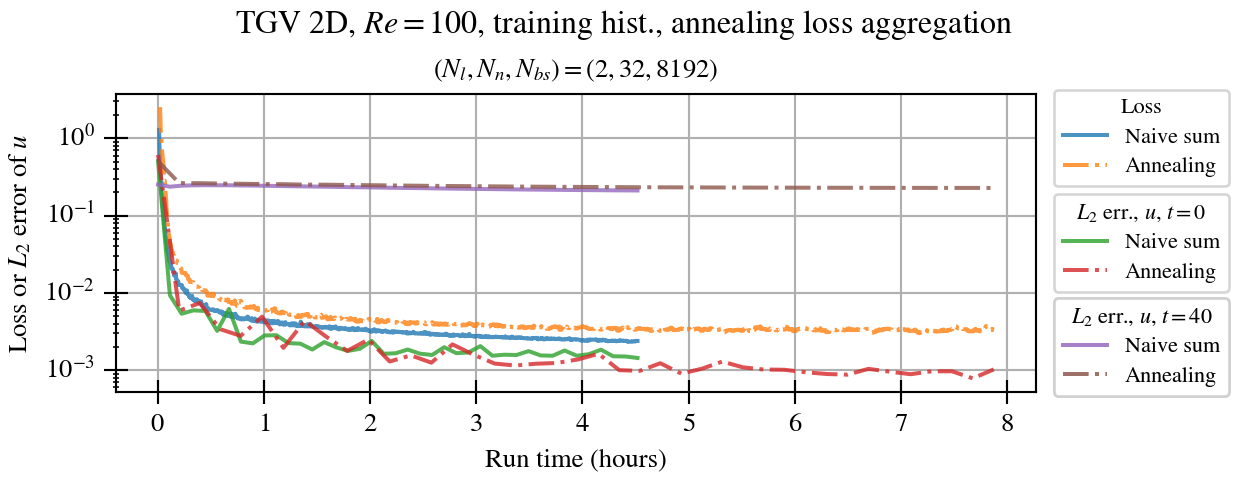
\includegraphics[width=0.9\linewidth]{tgv-2d-re100/annealing-tests/nl2-nn32-npts8192-walltimes}%
    \caption[%
        Annealing loss aggregation: loss and $L_2$ errors of $u$ v.s. wall time ($(N_l, N_n, N_{bs})=(2, 32, 8192)$)%
    ]{%
        Annealing loss aggregation: loss and $L_2$ errors of $u$ v.s. wall time ($(N_l, N_n, N_{bs})=(2, 32, 8192)$)%
    }\label{fig:annealing-tests-nl2-nn32-npts8192-walltimes}%
\end{figure}

\begin{figure}[hbt!]
    \centering%
    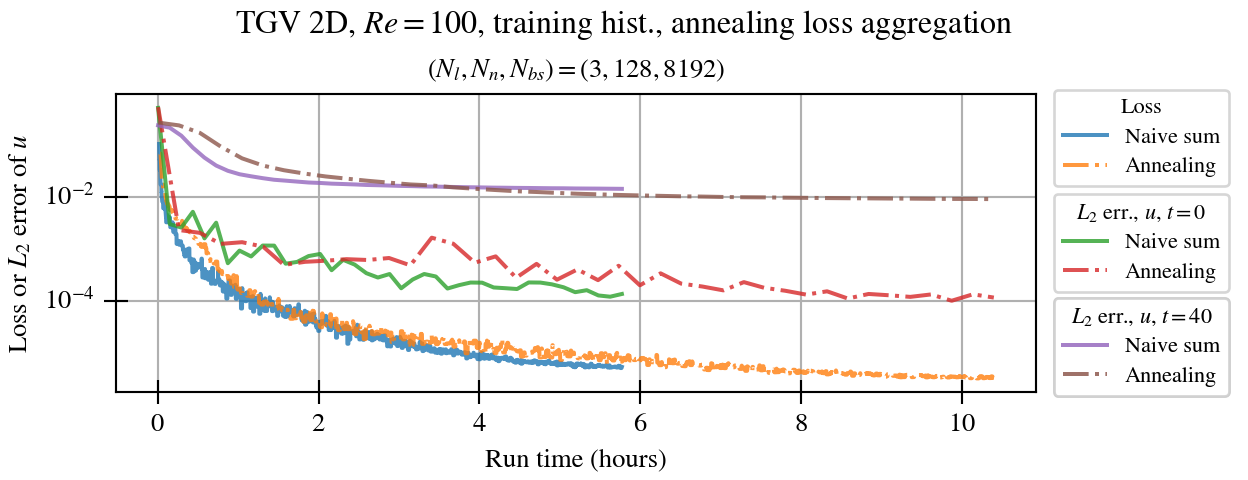
\includegraphics[width=0.9\linewidth]{tgv-2d-re100/annealing-tests/nl3-nn128-npts8192-walltimes}%
    \caption[%
        Annealing loss aggregation: loss and $L_2$ errors of $u$ v.s. wall time ($(N_l, N_n, N_{bs})=(3, 128, 8192)$)%
    ]{%
        Annealing loss aggregation: loss and $L_2$ errors of $u$ v.s. wall time ($(N_l, N_n, N_{bs})=(3, 128, 8192)$)%
    }\label{fig:annealing-tests-nl3-nn128-npts8192-walltimes}%
\end{figure}

\subsubsection{Cyclical Learning Rate and Stochastic Weight Averaging}

The benchmarks in this section cover the cyclical learning rate and stochastic weight averaging (SWA).
The cyclical learning rate (equation \eqref{eq:cyclical-learning-rate}) in this section was configured with $\eta_{low}=1.5e-5$, $\eta_{high}=1.5e-3$, $N_c=5000$, and $\gamma=0.999989$.
Figure \ref{fig:cyclic-swa-tests-lr-hist} shows a comparison of the learning rate from the original exponentially-decaying and the cyclical learning rate.
\begin{figure}[hbt!]
    \centering%
    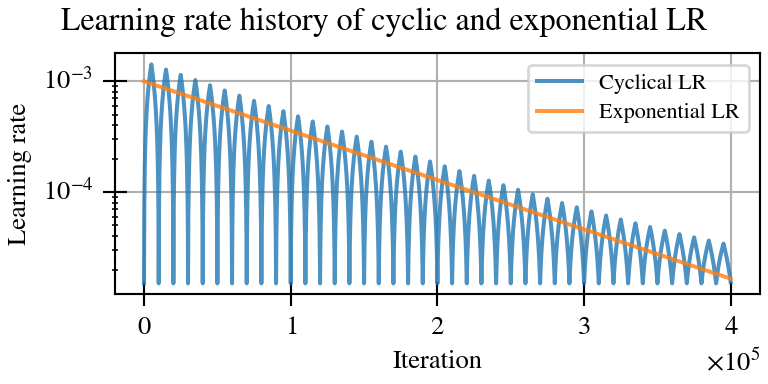
\includegraphics{tgv-2d-re100/cyclic-swa-tests/learning-rate-hist}%
    \caption[%
        Cyclical LR and SWA: learning rate history%
    ]{%
        Cyclical LR and SWA: learning rate history%
    }\label{fig:cyclic-swa-tests-lr-hist}%
\end{figure}
The exponentially-decaying learning rate will be simply denoted as {\it exponential} learning rate in the later discussion and figures.
SWA, on the other, hand, runs in parallel when using cyclical learning rate and does not affect the normal training process.
It is thus able to decouple the performance of SWA from the results of only cyclical learning rate.
In the cases presented here, SWA was configured to collect and average the model parameters from the last 200,000 iterations of the training.
Its results share the same convergence histories with the cases of pure cyclical learning rates.
The only difference between with and without SWA lies in the prediction errors (e.g., errors in $u$) after iteration 200,000.

\begin{figure}[hbt!]
    \centering%
    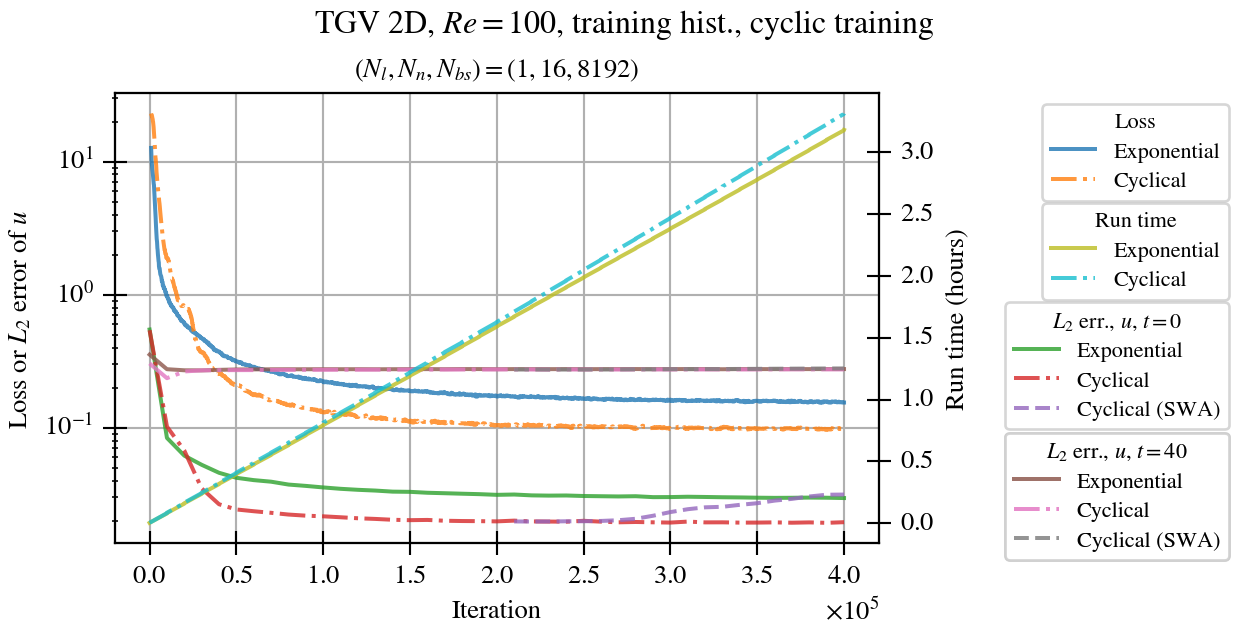
\includegraphics[width=0.9\linewidth]{tgv-2d-re100/cyclic-swa-tests/nl1-nn16-npts8192}%
    \caption[%
        Cyclical LR and SWA: loss and $L_2$ errors of $u$ v.s. iteration ($(N_l, N_n, N_{bs})=(1, 16, 8192)$)%
    ]{%
        Cyclical LR and SWA: loss and $L_2$ errors of $u$ v.s. iteration ($(N_l, N_n, N_{bs})=(1, 16, 8192)$)%
    }\label{fig:cyclic-swa-tests-nl1-nn16-npts8192}%
\end{figure}

\begin{figure}[hbt!]
    \centering%
    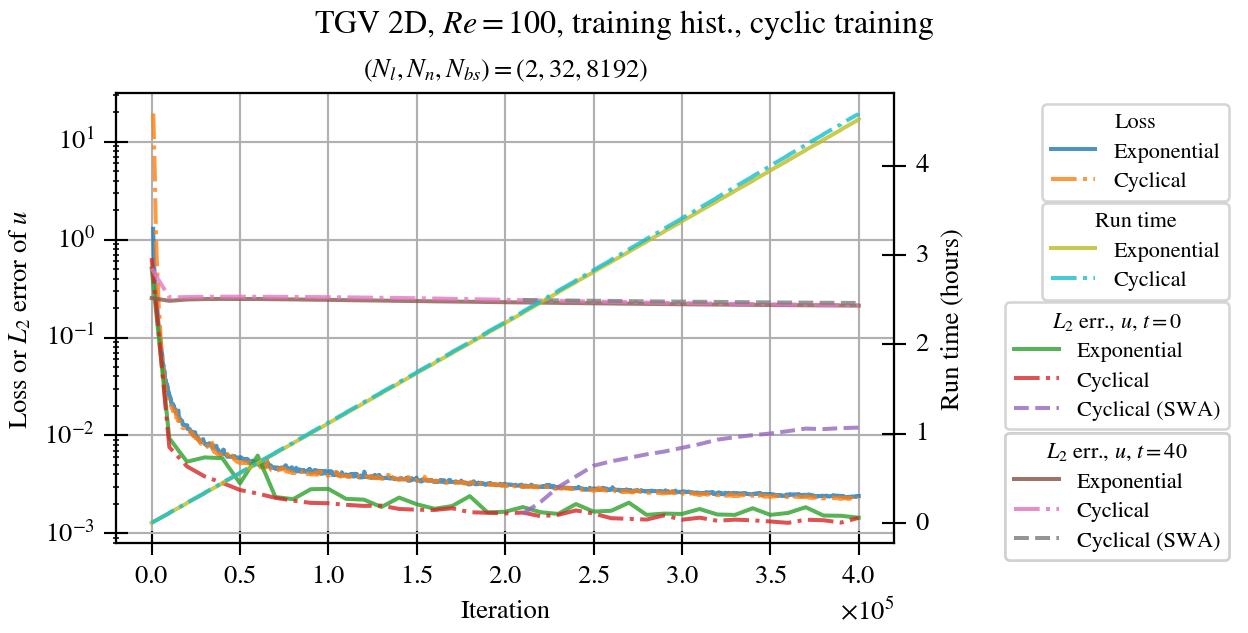
\includegraphics[width=0.9\linewidth]{tgv-2d-re100/cyclic-swa-tests/nl2-nn32-npts8192}%
    \caption[%
        Cyclical LR and SWA: loss and $L_2$ errors of $u$ v.s. iteration ($(N_l, N_n, N_{bs})=(2, 32, 8192)$)%
    ]{%
        Cyclical LR and SWA: loss and $L_2$ errors of $u$ v.s. iteration ($(N_l, N_n, N_{bs})=(2, 32, 8192)$)%
    }\label{fig:cyclic-swa-tests-nl2-nn32-npts8192}%
\end{figure}

\begin{figure}[hbt!]
    \centering%
    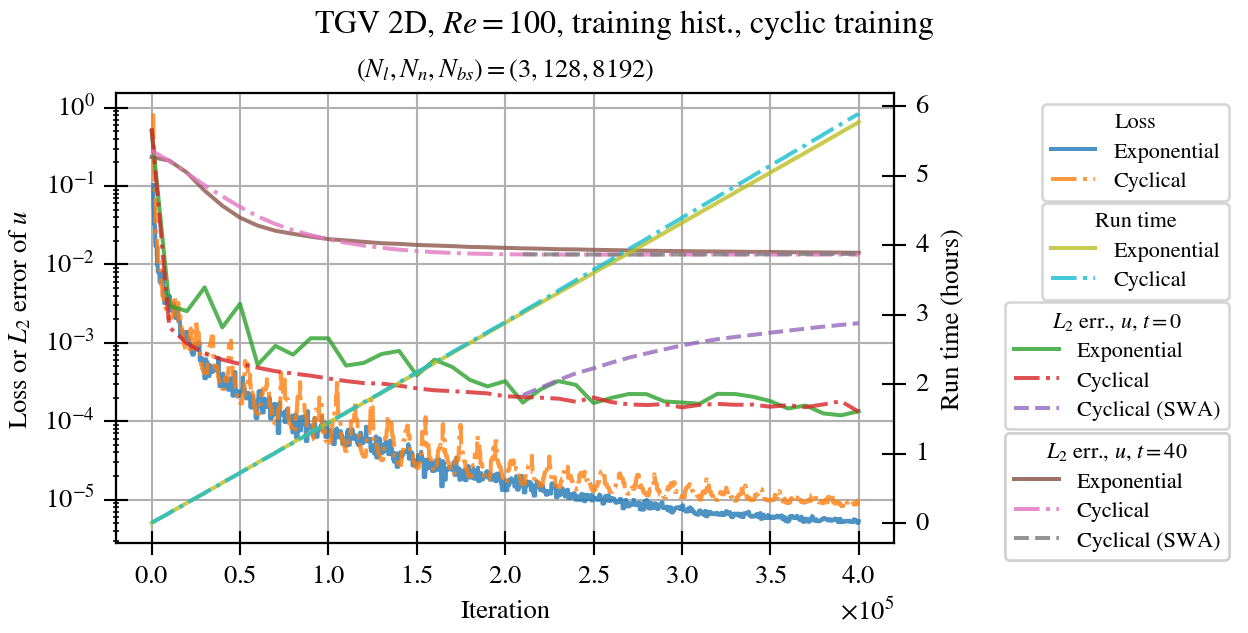
\includegraphics[width=0.9\linewidth]{tgv-2d-re100/cyclic-swa-tests/nl3-nn128-npts8192}%
    \caption[%
        Cyclical LR and SWA: loss and $L_2$ errors of $u$ v.s. iteration ($(N_l, N_n, N_{bs})=(3, 128, 8192)$)%
    ]{%
        Cyclical LR and SWA: loss and $L_2$ errors of $u$ v.s. iteration ($(N_l, N_n, N_{bs})=(3, 128, 8192)$)%
    }\label{fig:cyclic-swa-tests-nl3-nn128-npts8192}%
\end{figure}

In figures \ref{fig:cyclic-swa-tests-nl1-nn16-npts8192}, \ref{fig:cyclic-swa-tests-nl2-nn32-npts8192}, and \ref{fig:cyclic-swa-tests-nl3-nn128-npts8192}, we presented the convergence histories and the time costs.
First, the run times between the two learning rate strategies are similar.
This is expected as cyclical learning rate does not add notable operations to the training.

We next examined the convergence of cyclical and exponentially-decaying learning rates.
The results show that obvious difference only exists in the simplest model, $(1, 16, 8192)$.
However, this difference may be obvious only because the narrower $y$-axis scale in figure \ref{fig:cyclic-swa-tests-nl1-nn16-npts8192}.
If we plot all three figures using the same scale, the difference in $(1, 16, 8192)$ may not be noticeable.
The quantitative difference also supports this claim.
For example, the final loss of exponential learning rate is about $2e-1$, and that of cyclical learning rate is around $1e-1$.
We do not consider this difference significant.

Also, slight oscillation and evident oscillation can be seen in $(2, 32, 8192)$ and $(3, 128, 8192)$, respectively. 
The oscillations may represent how cyclical learning rate helps in escaping local minimums and saddle points. 
The reason that $(1, 16, 8192)$ does not show oscillation may be attributed to the simple hypersurface of $r(\Theta)$.
This architecture may be too simple and may not exhibit complex topography on the hypersurface.

The results in the errors of $u$ show that SWA does not help achieve better predictions at all.
It even hurts the prediction accuracy for $t=0$.
As for $t=40$, for reasons unknown to us at this point, there is no difference.
However, as there is no theory nor guidelines to determine how many iterations should be involved in SWA, the results may be different if using fewer iterations.
Although in this work we did not investigate more on SWA, it could be a potential research question for future studies.

\begin{figure}[hbt!]
    \centering%
    \includegraphics[width=0.9\linewidth]{tgv-2d-re100/cyclic-swa-tests/final-spatial-temporal-errors}%
    \caption[%
        Cyclic LR and SWA: final spatial-temporal errors%
    ]{%
        Cyclic LR and SWA: final spatial-temporal errors%
    }\label{fig:cyclic-swa-tests-final-sterrs}%
\end{figure}

Figure \ref{fig:cyclic-swa-tests-final-sterrs} shows the graphical comparison of the overall spatial-temporal error, $L_{2,sp-t}$.
The results are similar.
Even though SWA gives worse predictions at $t=0$, the integrated error over $t=0$ to $t=100$ does not show significant difference.

\subsubsection{Nonlinear Conjugate-Gradient Optimizer}
\label{sec:ncg-tests}

The last attempt to adopt new training strategy was the application of nonlinear conjugate-gradient.
The major difficulty of applying CG lies in how to handle batch training.
CG relies on the previous search direction to determine the current search direction, and the former is based on the hypersurface in the last iteration.
In batch training, the hypersurface more or less changes from iteration to iteration due to using different training points.
It is unclear how legit the previous search direction is to be used in the current iteration.

Moreover, in each iteration, the line search algorithm search for a new location along the search direction according to the Wolfe conditions or their derived conditions.
A point meets the Wolfe conditions in the previous iteration does not necessarily meet the same conditions in the current iteration.
This may cause convergence issues in CG as the convergence of CG relies on properly determining the location on each search direction.

Nevertheless, given the efficiencies of CG in non-batched training, we would like to experiment the possibility of using it.
In our current attempt, we used CG to optimize the loss $r(\Theta)$ for a certain batch to a given tolerance before moving on to the next batch.
Also, CG may not have capability to escape from poor local minimums, so our attempts first used Adam for optimization up to 200,000 iterations to identify a region with proper minimum, and then CG was used for an extra 200 iterations.
In other words, pure Adam cases ran 400,000 iterations, while the CG cases ran 200,000 Adam iterations and then 200 iterations with CG.
The case tested are $(1, 16, 8192)$, $(2, 32, 8192)$, and $(3, 128, 8192)$.
CG trained each batch until the change in the loss is smaller than $1e-6$.

\begin{figure}[hbt!]
    \centering%
    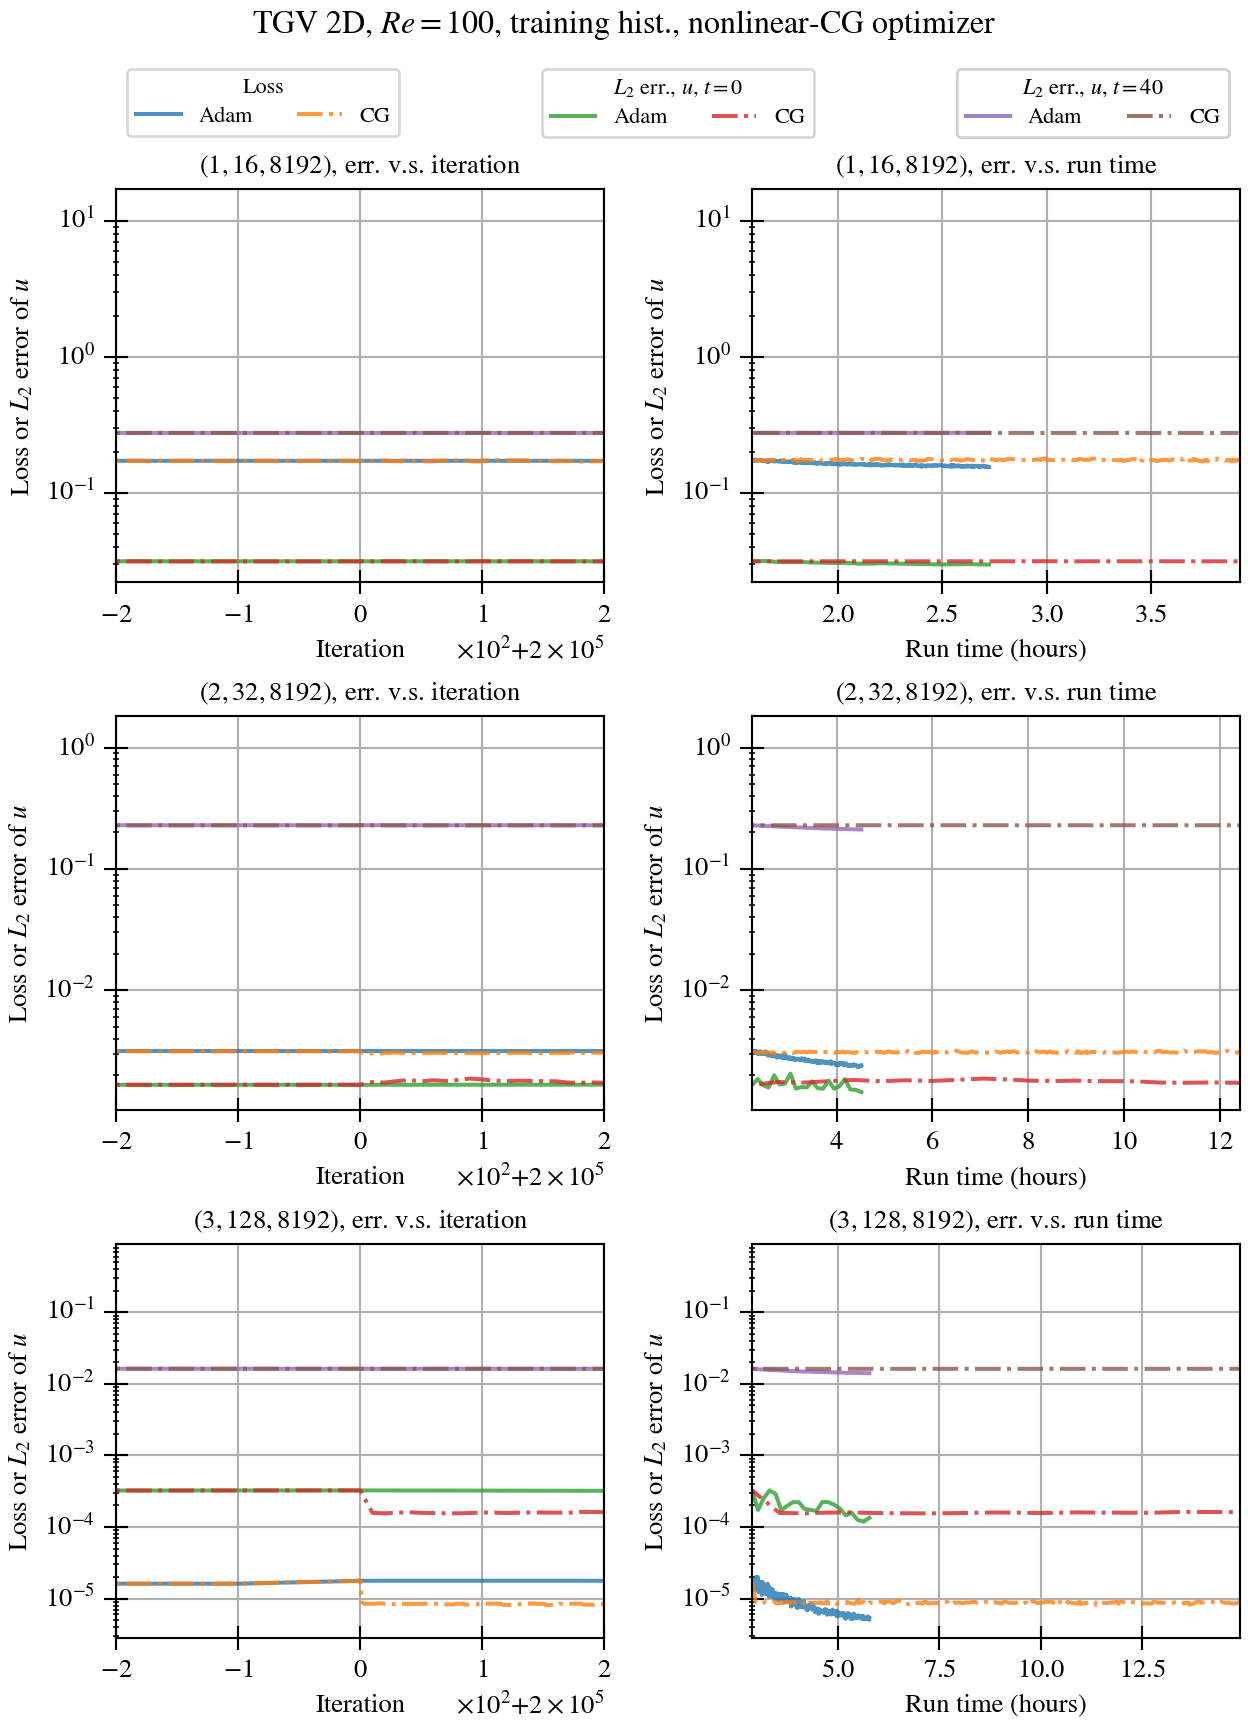
\includegraphics[width=\linewidth]{tgv-2d-re100/ncg-tests/training-hist}%
    \caption[%
        Nonlinear-CG: training history%
    ]{%
        Nonlinear-CG: training history%
    }\label{fig:ncg-tests-train-hist}%
\end{figure}

Figure \ref{fig:ncg-tests-train-hist} shows the comparison of convergence histories between Adam-only cases and CG cases.
On the left we have the losses and errors versus iterations.
The range of iterations shown in the $x$-axis is 199,800th to 200,200th iteration.
We can see for simple architectures, CG does not help reduce the losses.
Based on the observations and discussions in the previous sections, cases with simple architectures converge very early.
It is hence reason for CG not able to improve the losses in simple architectures because they may have already converged.
However, $(3, 128, 8192)$ does show a sudden drop in the loss and error at $t=0$.
After the sudden drop, further training with new batches does not further improve the loss and errors.

On the right of the same figure, we have losses and errors versus run time.
The range of the run time starts from the time for 200,000 iterations until the end of training.
In other words, sub-figures on the right show the 200,000th to 400,000th training iterations for Adam-only cases and 200,000th to 200,200th training iterations for CG cases.
As we use CG on each batch until a certain tolerance, one training iteration with CG consists of hundreds or thousands of sub-iterations inside the CG solver.
Therefore, it is reasonable to see 200 training iterations with CG takes much longer time than 200,000 iterations with Adam.
It is clear from these sub-figures, although CG provides a sudden drop in the losses, it does not further improve the training.
And eventually, Adam reaches even smaller losses than CG does.
More importantly, Adam take much less time.

\begin{figure}[hbt!]
    \centering%
    \includegraphics[width=0.9\linewidth]{tgv-2d-re100/ncg-tests/final-spatial-temporal-errors}%
    \caption[%
        Nonlinear-CG: overall spatial-temporal errors%
    ]{%
        Nonlinear-CG: overall spatial-temporal errors%
    }\label{fig:ncg-tests-final-sterrs}%
\end{figure}

Figure \ref{fig:ncg-tests-final-sterrs} shows the final spatial-temporal errors of $u$ and $v$ velocity.
CG does not provide more accurate results.

As mentioned, the major problem with CG is the combined use with batch training and the capability to escape from saddle points and poor minimums.
Carefully tuned line search parameters and algorithm may help achieve the escaping.
However, how to deal with batched training is still a question.
If the issues is caused by the change in hypersurface, then using more training points per batch may help stabilize the hypersurface from iteration to iteration.
And hence each CG iteration is itself a training iteration, i.e., each batch of points is used in one CG iteration.
This may be a potential direction for future investigation on this topic.
% vim:ft=tex